
\chapter{弹性及其应用}

弹性衡量买者与卖者对市场条件变化的反应程度。

\section{需求弹性}

\subsection{需求价格弹性及其决定因素}

\keyword{需求价格弹性}衡量需求量对价格变动的反应程度。
如果一种物品的需求量对价格变动的反应很大,
就说明这种物品的需求量是\keyword{富有弹性}的。
如果一种物品的需求量对价格变动的反应很小,
就说明这种物品的需求是\keyword{缺乏弹性}的。


由于需求反映了形成消费者偏好的许多经济、社会与心理因素,
所有没有一个决定需求曲线弹性的简单而普遍的规律。
但根据经验,我们可以总结出某些决定需求价格弹性的经验法则。

\begin{description}
\item[相似替代品的可获得性] 有相似替代品的物品的需求往往较富有弹性。
\item[必需品与奢侈品] 必需品的需求往往缺乏弹性,而奢侈品的需求往往富有弹性。
\item[市场的定义] 任何一个市场上的需求弹性都取决于我们如何划定市场的边界。狭窄定义的市场的需求弹性往往大于宽泛定义的市场的需求弹性,因为狭窄定义的市场长的物品更容易找到相近的替代品。
\item[时间范围] 物品的需求往往在长期内更富有弹性。
\end{description}



\subsection{需求价格弹性的计算}

\begin{equation}
  \text{需求价格弹性} = \frac{\text{需求量变动百分比}}{\text{价格变动百分比}}
\end{equation}



\subsection{中点法:一个计算变动百分比和弹性的更好方法}

计算$(Q_1,P_1)$和$(Q_2,P_2)$两点间需求价格弹性的中点法可以用以下公式表示:
\begin{equation}
  \text{需求价格弹性} =
  \frac{
    \frac{Q_2-Q_1}{(Q_2+Q_1)/2}
  }{
    \frac{P_2-P_1}{(P_2+P_1)/2}
  }
\end{equation}


\subsection{各种需求曲线}

经济学家根据需求弹性对需求曲线进行分类。
当弹性大于1,需求是富有弹性的。
当弹性小于1,需求是缺乏弹性的。
当弹性等于1,需求是单位弹性的。



通过某一点的需求曲线越平坦,
需求价格弹性就越大;
通过某一点的需求曲线越陡峭,
需求价格弹性就越小。



\subsection{总收益与需求价格弹性}

\begin{figure}[!ht]
  \centering
  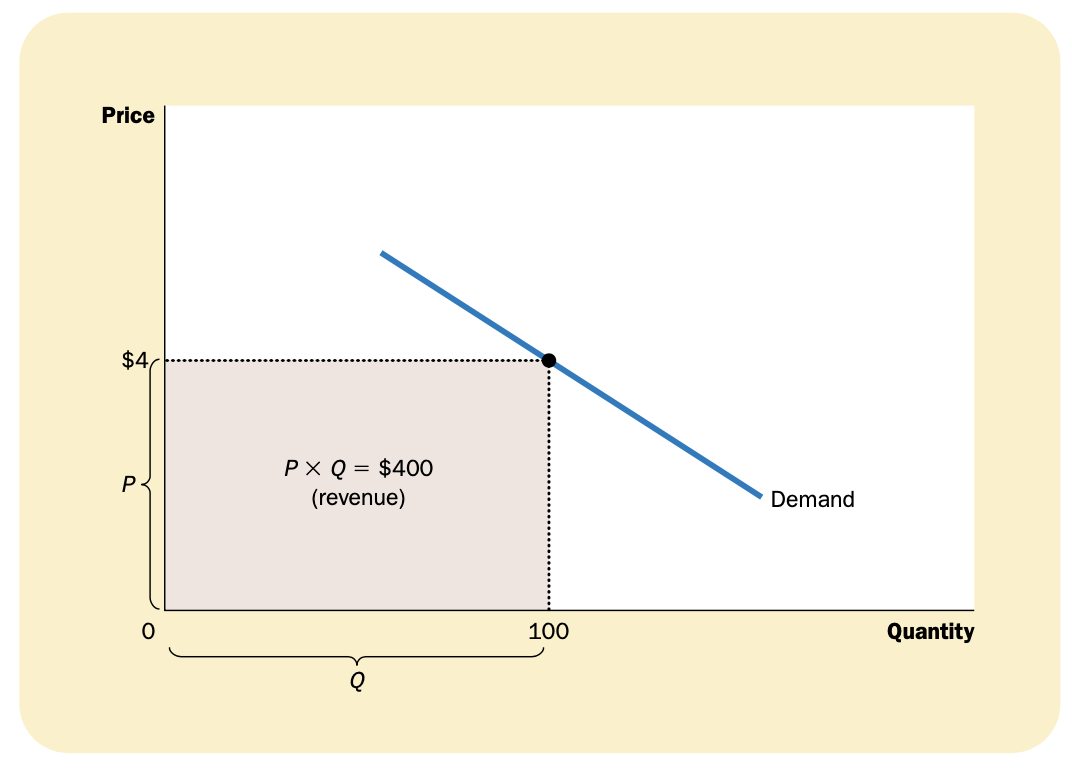
\includegraphics[width=\textwidth]{pics/total-revenue}
  \caption{总收益}
  \label{fig:total-revenue}
\end{figure}
如图\ref{fig:total-revenue}所示,
总收益是某种物品的买者支付从而卖者得到的量。
在任何一个市场上,总收益是$P\times Q$,
即一种物品的价格乘以该物品的销售量。


总收益如何沿着需求曲线变动呢?
答案取决与需求价格弹性。

\begin{figure}[!ht]
  \centering
  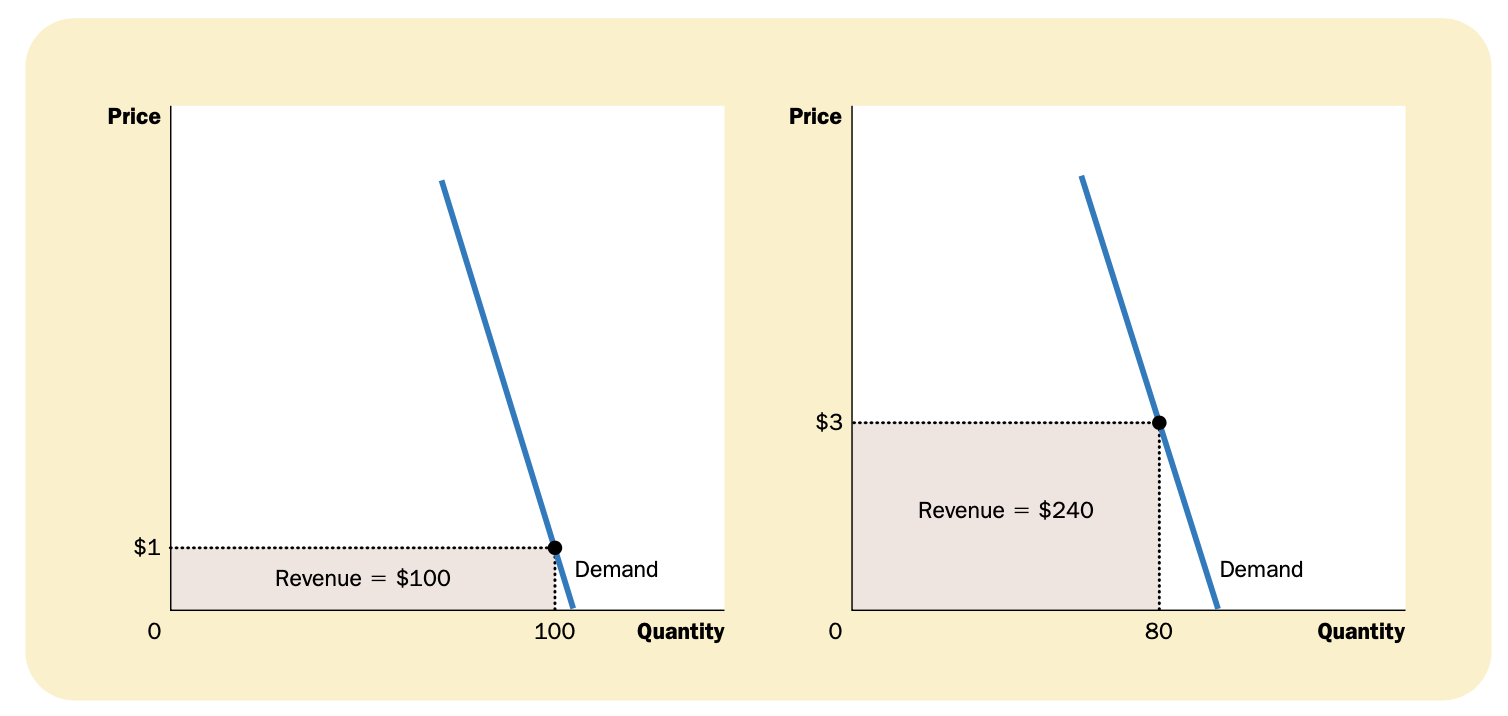
\includegraphics[width=\textwidth]{pics/inelastic-demand}  
  \caption{缺乏弹性}
  \label{fig:inelastic-demand}
\end{figure}

\begin{figure}[!ht]
  \centering
  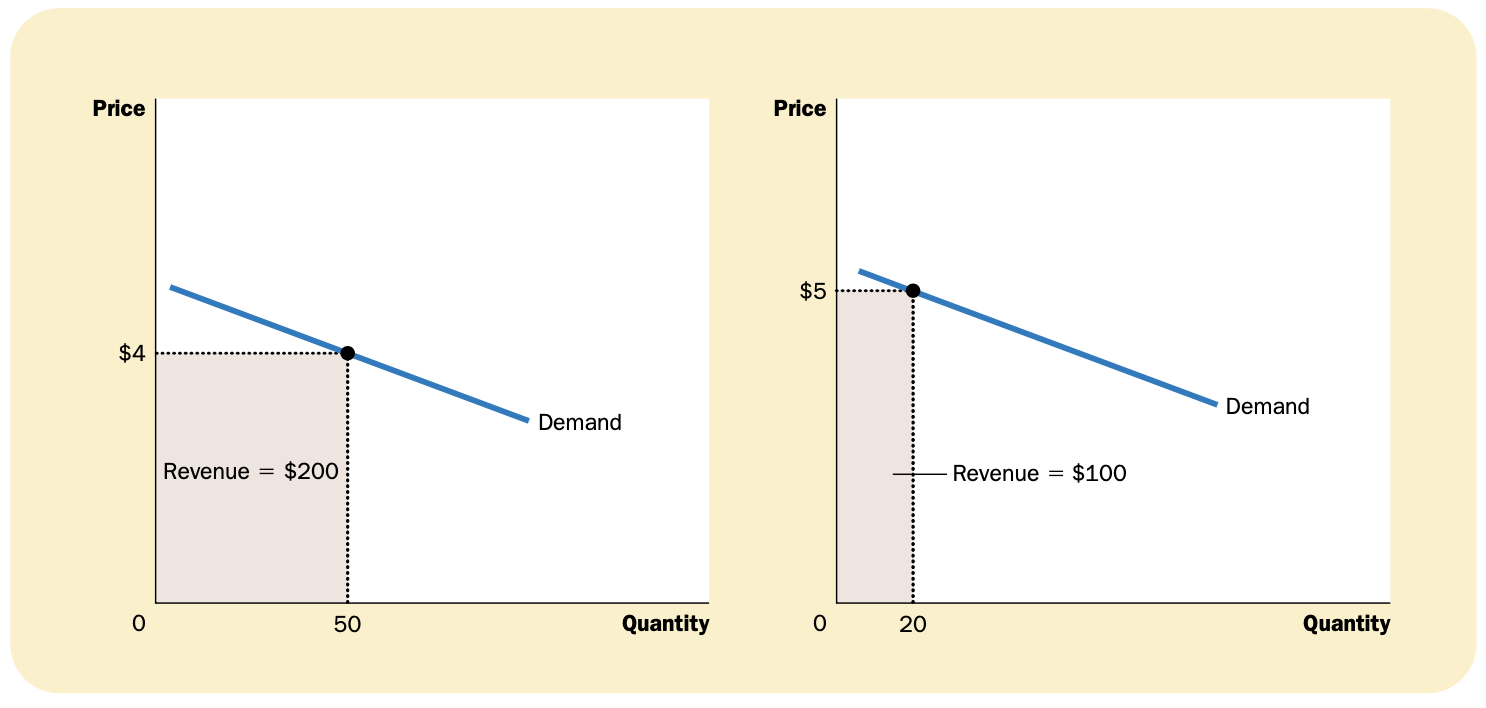
\includegraphics[width=\textwidth]{pics/elastic-demand}  
  \caption{富有弹性}
  \label{fig:elastic-demand}
\end{figure}


\begin{enumerate}
\item 当需求缺乏弹性(价格弹性小于1)时,价格和总收益同方向变动:如果价格上升,总收益增加。
\item 当需求缺乏弹性(价格弹性大于1)时,价格和总收益反方向变动:如果价格上升,总收益减少。
\item 如果需求是单位弹性的(价格弹性等于1)时,当价格变动时,总收益保持不变。
\end{enumerate}



\subsection{其他需求弹性}

\begin{equation}
  \text{需求收入弹性} = \frac{\text{需求量变动百分比}}{\text{收入变动百分比}}
\end{equation}

\begin{equation}
  \text{需求的交叉价格弹性} = \frac{\text{物品1的需求量变动百分比}}{\text{物品2的价格变动百分比}}
\end{equation}


\section{供给弹性}

\subsection{供给价格弹性及其决定因素}

\keyword{供给价格弹性}衡量供给量对价格变动的反应程度。
供给在长期中的弹性通常大于短期。


\subsection{供给价格弹性的计算}

\begin{equation}
  \text{供给价格弹性} = \frac{\text{供给量变动百分比}}{\text{价格变动百分比}}
\end{equation}


\subsection{各种供给曲线}

\begin{figure}[!ht]
  \centering
  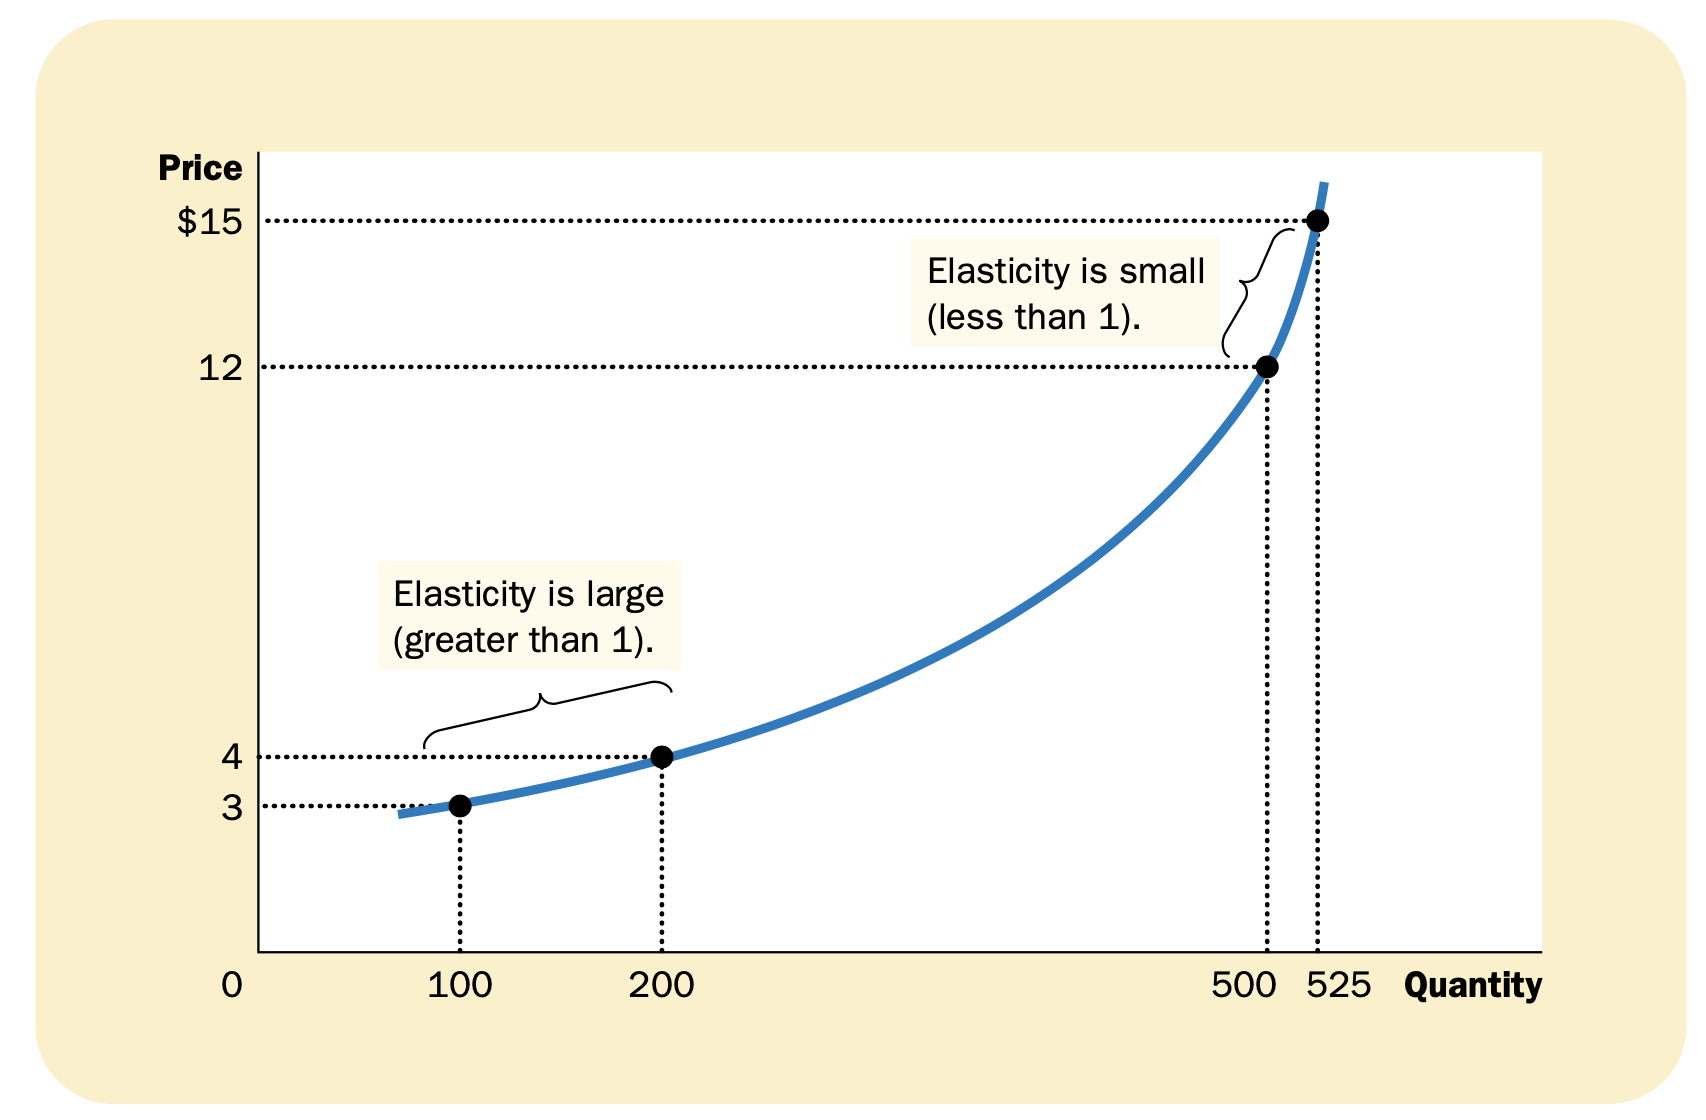
\includegraphics[width=\textwidth]{pics/supply-elastic-price}
  \caption{供给价格弹性的变动}
  \label{fig:supply-elastic-price}
\end{figure}



\section{供给、需求和弹性的应用}

\subsection{农业的好消息可能对农民来说是坏消息吗?}

\begin{figure}[!ht]
  \centering
  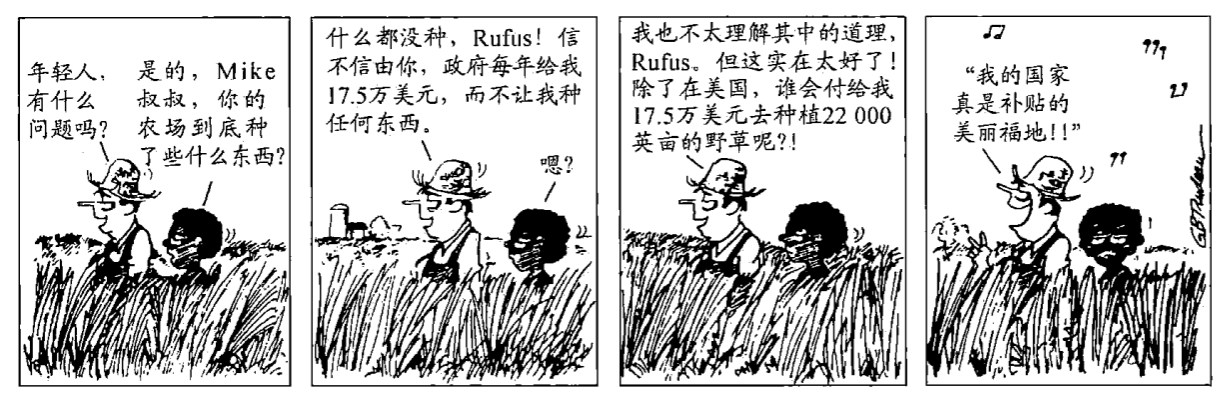
\includegraphics[width=\textwidth]{pics/farmer}
\end{figure}


对农民有力的不一定对整个社会也有利。
农业技术进步对农民而言可能是坏事,
因为它使农民逐渐变得不必要,
但对能以低价买到消费正而言可定是好事。
同样,旨在减少农产品供给的政策可以增加农民的收入,
但必然会以损害消费者的利益为代价。


\section{结论}

只要学会说“供给与需求”,甚至连一只鹦鹉都可能称为一个经济学家。